\documentclass{article}
\usepackage{graphicx}
\usepackage{wrapfig}
\usepackage{subcaption}
\usepackage[margin=1in]{geometry}
\usepackage{amsmath} % or simply amstext
\usepackage{amssymb}
\usepackage{siunitx}
\usepackage{booktabs}
\usepackage[export]{adjustbox}
\newcommand{\angstrom}{\textup{\AA}}
\newcommand{\colormap}{jet}  % colorbar to use
\usepackage{cleveref}
\usepackage{booktabs}
\usepackage{gensymb}
\usepackage{float}

\title{Statistical Inference of Transport Mechanisms and Long Time Scale Behavior from Time Series 
       of Solute Trajectories in Nanostructured Membranes.}

\author{Benjamin J. Coscia, Christopher P. Calderon \and Michael R. Shirts} 

\begin{document}

  \graphicspath{{./figures/}}
  \maketitle
  
  % BJC2: I'm not putting a lot of effort into the introduction since I'll only write
  % an abbreviated form for my dissertation. I'll work on the intro after my defense.  

  \section{Introduction}
  
  There is a need for highly selective membranes in order to perform efficient 
  separations of components of complex aqueous streams.
  %MRS2: add some more examples (When you get around to it).
  \begin{itemize}
    \item Organic micropollutants
    \item Desalination and boric acid removal from seawater.
    \item While many researchers focus on membrane permeability, we may be 
    able to reduce costs of commercial nanofiltration and reverse osmosis with
    higher selectivity.~\cite{werber_materials_2016}
  \end{itemize}

%  \noindent Amphiphilic molecules are capable of self-assembling into ordered nanostructures.
%  \begin{itemize}
%    \item 
%  \end{itemize}

  Lyotropic liquid crystals (LLC) are a class of amphiphilic molecules whose ordered phases
  can be cross-linked into mechanically strong membranes capable of highly selective
  separations.
  \begin{itemize}
    \item The shape of the LLC monomers and water content dictates the ordered phase 
    that they form. There are two phases of particular interest for membrane applications.
  	\item H\textsubscript{II} phase lyotropic liquid crystals are characterized by 
  	hexagonally packed, straight, pores while the Q\textsubscript{I} phase consists of
  	a tortuous network of 3D interconnected pores. 
  	\item In both cases the pores are uniform in size with radii on the order of 1 nm
    %MRS2: is it really a molecular weight cutoff?
    %BJC2: is molecular size better? Obviously there are other factors like shape, but I don't want to get into that
  	giving them a very strict molecular size cut-off.
	\item Additionally, they have the potential to disrupt conventional membrane separation
	techniques by being selective based not only on size and charge, but on chemical
	functionality as well.
	\item Their pores are lined with LLC monomer functional groups which can potentially
	be designed to interact with solutes in a chemically-specific manner
  \end{itemize}

  There are limits to what we can learn from experiment about LLC membrane design.
  \begin{itemize}
    \item Experimental observables like permeability and selectivity allow us to speculate
    about the molecular origins of separation processes.
    %MRS2: not quite sure what you mean below?
    \item This drives an empirical design approach which can potentially neglect key
    interactions which influence selectivity.
    \item LLC membranes have been shown to exhibit selectivities which cannot be fully 
    explained by relatively simple macroscopic models. 
  \end{itemize}
  
  Molecular Dynamics (MD) simulations can give us mechanistic insights with atomistic 
  resolution so that we can intelligently design new membranes for solute-specific 
  separations.
  \begin{itemize}
    \item In our previous work, we built a detailed atomistic model which we used
    to understand the nanoscopic structure of an LLC Membrane.~\cite{coscia_understanding_2019}
    \item We also used the model in order to gain a qualitative understanding of 
    trapping mechanisms which lead to subdiffusive transport behavior.~\cite{coscia_chemically_2019}
  \end{itemize}

  Unfortunately, the timescales that we can simulate with MD are insufficient to be
  able to make well-converged predictions of macroscopic transport properties 
  traditionally used to characterize membranes in the lab.
  \begin{itemize}
    %MRS2: would be good to get this next point into the first line of a paragraph, since it's quite important. 
    \item However, if we use descriptive stochastic models that can capture solute
    dynamics, then we could project long timescale behavior in addition to gaining
    a deeper understanding of solute behavior on short timescales.
  \end{itemize}
  
  In our previous work, we designed two different approaches which used
  solute time series in order to parameterize stochastic models that could be used
  to project transport on much longer timescales.
  \begin{itemize}
  	\item In our first approach we modeled solute trajectories as subordinated fractional
  	Brownian and L\'evy motion, called the anomalous diffusion (AD) model. 
  	\item We generated solute trajectories by generating a series
  	of anti-correlated hops separated by random periods of entrapment drawn from a 
  	power law distribution.
  	\item Our second approach treated solute motion as a Markov state model with
  	state-dependent dynamics, called the Markov state-dependent dynamical model (MSDDM).
  	\item We parameterized the state transition probabilities between
  	each of eight discrete states as well as the solute dynamics within each of these
  	states. We generated stochastic trajectory realizations by drawing a state
  	sequence based on the transition probability matrix and incorporating the state dynamics
  	while solutes were trapped in each state.
%  	\item Both models had moderate success reproducing the mean squared displacements (MSDs)
%  	exhibited by solutes in our MD simulations.
  \end{itemize}
  
  Although both models had reasonable success at predicting solute mean squared 
  displacements (MSDs) on MD simulation timescales, they had shortcomings.
  \begin{itemize}
  	\item The MSDDM failed to reproduce the hopping and trapping behavior that
  	characterizes solute center-of-mass trajectories in our MD simulations.
  	\item The AD model did not suffer this qualitative shortcoming, but the 
  	persistent curvature of the predicted MSD curves suggested that the model
  	might underestimate MSDs on long timescales. 
  	\item The formulation of both models required careful examination and
  	characterization of the interactions and dynamics exhibit by MD trajectories 
  	which required considerable human effort.
  \end{itemize}
  
  % BJC: Not sure whether to call it the infinite hidden markov model or hierarchical dirichlet process hidden markov model
  % The former is definitely simpler.
  % MRS: True.  I would probably see which is used more in the literature. 
  % BJC1: going with IHMM. HDPHMM seems to mostly be used by Emily Fox
  In this work, we apply the infinite hidden Markov Model (IHMM), a modeling
  approach that is agnostic to the source of time series data, in order to 
  automatically detect and infer the parameters of an unknown number of latent
  autoregressive (AR) modes present in solute center-of-mass time series.
  \begin{itemize}
  	\item In addition to AR parameters for each state, the IHMM estimates the
  	state transition probability matrix.
  	\item The model helps simultaneously uncover underlying transport mechanisms which
  	give rise to dynamical behavior and project that behavior on longer timescales so
  	that we can estimate macroscopic transport observables.
  \end{itemize}
  
  We use the parameters of the states identified by the IHMM in order to infer 
  dominant solute-membrane interactions and transport mechanisms.
  \begin{itemize}
    \item We compare the inferred mechanisms to those which we manually
    identified in our previous work. 
    %MRS2: don't put the conclusions in the introduction.  Instead, state clearly the questions you will ask and the hypotheses you will test.
   \item Some kind of conclusion here. Did we find more or less states. Any new states/ subdivisions of states?
  \end{itemize}
  
  We can also use the IHMM to generate stochastic trajectory realizations that share
  the same dynamical characteristics as solute trajectories observed in our MD 
  simulations. 
  \begin{itemize}
    \item The trajectories are qualitatively similar, showing expected hopping and trapping
    behavior.
    \item They are quantitatively similar in that they reproduce the MSDs measured in MD.
  \end{itemize}

  Finally, we use the stochastic trajectory realizations in order to compute the 
  macroscopic flux of each solute and selectivity of the LLC membranes studied towards
  each solute.
  \begin{itemize}
    %MRS2: shouldn't reach conclusions in intro, just set up questions to be answered (conclusions SHOULD be in abstract).
    \item We relate these macroscopic properties to our nanoscopic model by simulating 
    mean first passage time (MFPT).
    \item Some kind of conclusion. This membrane is selective towards solutes with this
    functionality. 
    \item Does the conclusion agree with our previous work? Any length dependence? (I think not)
  \end{itemize}
    
  \section{Methods}
    
  We ran all MD simulations and energy minimizations using GROMACS 2018. We
  performed all post-simulation trajectory analysis using python scripts which are available
  online at \\ \texttt{https://github.com/shirtsgroup/LLC\_Membranes}.

  \subsection{Molecular Dynamics Simulations}
  
  % BJC: Could I just reference previous work here? "MD simulations were run as 
  % described in our previous work..."
  % BJC2: Or I could just say that I'm using the same data from the last paper. See that paper.

  We studied transport of solutes in the H\textsubscript{II} phase using an
  atomistic molecular model of four pores in a monoclinic unit cell with 
  10 \% water by weight. 
  \begin{itemize}
    \item Approximately one third of the water molecules occupy the tail region 
    with the rest near the pore center.
    \item We chose to study the 10 wt \% water system because solutes move 
    significantly faster than in the 5 wt \% system studied previously.
    \item Appropriate stochastic modeling requires that solutes sample the 
    accessible mechanisms with representative probability.%MRS: only possible on the ~1-10 \mu scale with relatively fast solutes.
  \end{itemize}
  
  We chose to study a subset of 4 of the fastest moving solutes from our previous
  work: methanol, acetic acid, urea and ethylene glycol.
  \begin{itemize} 
    \item In addition to exploring membrane structural space the most, these solutes
    have a relatively diverse set of chemical functionality.   
    \item For each solute we created a separate system and to each system we
    added 6 solutes per pore for a total of 24 solutes.
    \item This number of solutes per pore provides a balance of a low 
    degree of interaction between solutes and sufficient amount of data from
    which to generate statistics on the time scales which we simulate.
    \item Further details on the setup and equilibration of these systems can
    be found in our previous work.\cite{coscia_chemically_2019}
  \end{itemize}
  
  \noindent We extended the 1 $\mu$s simulations of our previous work to 5 $\mu$s in order
  to collect ample data.
  \begin{itemize}
    \item We simulated the system with a time step of 2 fs at a pressure of 1 bar
    and 300 K controlled by the Parinello-Rahman barostat and the v-rescale thermostat
    respectively.
    \item We recorded frames every 0.5 ns
  \end{itemize}

  \subsection{The Infinite State Hidden Markov Model}\label{method:IHMM}
  
  Hidden Markov models (HMMs) are a useful and widely used technique
  for modeling sequences of observations where the probability of the next observation
  in a sequence depends, at least in part, on a previous unobserved, latent or hidden, state.~\cite{beal_infinite_2002}
  \begin{itemize}
    \item In the context of our simulations, the observations correspond to 
    the center of mass coordinates of the solutes versus time, and the states
    correspond to the dynamical behavior which give rise to those types
    of observations.
    \item The probability of transitioning to a state based on the current
    state is mathematically defined in terms of an $n\times n$ transition
    probability matrix, $T$, where $n$ is the number of states.
    \item Unfortunately, standard HMMs require $n$ to be known
    \textit{a priori}.
    \item One can partially overcome this by testing a range of numbers of 
    hidden states and determining which is the best representation of the
    data.
  \end{itemize}
  
  %BJC: I'm not sure how much of this I should include. This is pretty much 
  % a reproduction of Fox et al's explanation: https://ieeexplore.ieee.org/abstract/document/5563110
  The infinite-state HMM overcomes this drawback by placing a hierarchical
  Dirichlet process (HDP) prior on the transition probabilities.
  \begin{itemize}
    \item Using some base probability distribution, $H$, a Dirichlet process 
    (DP) generates discrete distributions, $G_0$, over a countably infinite 
    number of probability measures:
    \begin{equation}
      G_0 = \sum_{k=1}^{\infty} \beta_k \delta_{\theta_k} ~~ \theta_k \sim H, \beta \sim GEM(\gamma)
    \end{equation}
    where the $\theta_k$ are values drawn from the base distribution and the
    weights $\beta_k$ come from a stick-breaking process parameterized by the  
    concentration parameter $\gamma$ (equivalently referred to as GEM($\gamma$)). 
    \item Also expressed $G_0 \sim DP(\gamma, H)$
    \item The concentration parameter, $\gamma$, expresses one's confidence in the 
    base distribution $H$.
    \item We use a uniform base distribution.
    \item When $\gamma\to 0$, the first weight of $G_0$, $\beta_1$, approaches 
    unity and for $\gamma\to\infty$, the weights become uniform and $G_0$ closely
    resembles $H$.
    \item Each row, $G_j$, of the transition matrix is produced by drawing from a DP specified 
    using the $\beta$ vector as a discrete base distribution and a separate concentration
    parameter, $\alpha$.
    \begin{equation}
      G_j = \sum_{k=1}^{\infty} \pi_{jk} \delta_{\theta_k} ~~ \pi_j \sim DP(\alpha, \beta)
    \end{equation}
    \item This hierarchical specification ensures that the transition probabilities in 
    each row share the same support points \{$\theta_1$, ..., $\theta_k$\}.
    \item Once the model has converged only a finite number of states will have significant
    sampling.
  \end{itemize}
  
  We describe the dynamics of each state visited by solutes using a first order vector 
  autoregressive (VAR(1)) model. 
  \begin{itemize}
  	\item In general, a VAR($r$) process is characterized by a vector of observations in a time series 
  	that are linearly dependent on $r$ previous values of the time series vector:
  	\begin{equation}
  	\mathbf{y}_t = \mathbf{c} + \sum_{i=1}^r A_i\mathbf{y}_{t-i} + \mathbf{e}_t~~~~\mathbf{e}_t \sim \mathcal{N}(0, \Sigma)
  	\label{eqn:var}
  	\end{equation}
  	Previous observations are weighted by coefficient matrices, $A_i$. The VAR($r$) 
  	process is further characterized by a shift in the mean of each dimension by the
  	vector $\mathbf{c}$ and a white noise term $\mathbf{e}_t$.~\cite{hamilton_time_1994}
  	\item We assumed $\mathbf{e}_t$ to be multivariate Gaussian noise, with mean zero and
  	covariance, $\Sigma$.
  	\item We limited our analysis to an autoregressive order of $r=1$.
  	\item This means that we only parameterize $A_1$. To simplify notation, we will just
  	call it $A$.
  	\item We used a matrix-normal inverse-Wishart prior on parameters $A$ and $\Sigma$ 
  	and a Gaussian prior on $\mathbf{c}$ in order to infer their values.~\cite{fox_nonparametric_2009}
  	%BJC2: I'm not sure above is enough to make it clear how I got the parameters. Maybe I should
  	% explicitly refer to the fox paper above which outlines the inference procedure in more detail?
  \end{itemize}   
  
  % BJC2: It might be useful to walk through the following procedure with an example 
  % trajectory
  
  %Based on the algorithms developed by Fox et al.~\cite{fox_sticky_2007}, 
  Using the IHMM framework, we estimated the most likely number and sequence of hidden
  states in each solute center-of-mass trajectory while simultaneously inferring VAR(1)
  parameters for each state and the overall state transition probability matrix, $T$.
  \begin{itemize}
    \item We created a python implementation of this process which we heavily adapted from
    the MATLAB code of Fox et al.~\cite{fox_sticky_2007} 
    %BJC3: I got the software from this page: https://homes.cs.washington.edu/~ebfox/software/
    % Maybe I should reach out to emily fox to see how she would prefer I cite the software?
    %MRS4: yes, she how she wants to cite it.
    \item Parameter estimation is iterative. Therefore, we looked for convergence 
    of each entry in the $\mathbf{c}$ vector as well as the $A$ and $\Sigma$ matrices of 
    Equation~\ref{eqn:var}.
    \item We detected equilibration of the parameters using the module 
    \texttt{pymbar.timeseries.detect\_equilibration} on the time series of 
    parameter estimates. 
    \item Plots illustrating parameter convergence are available in the SI.
    \item We refer the interested reader to much more extensive descriptions of 
    the inference and sampling procedures used to estimate the VAR(1) parameters
    and the state sequence. 
    ~\cite{beal_infinite_2002,teh_hierarchical_2006,van_gael_beam_2008,fox_nonparametric_2009,fox_bayesian_2010}
  \end{itemize}

  We carefully applied the IHMM algorithm in a way which takes advantage of the
  system's cylindrical symmetry.
  \begin{itemize}
%    \item In general we are interested in the time series created by tracing
%    each solute's center of mass position. % ALready said this above
    \item There are a number of viable ways in which one could choose to analyze 
    these time series.
    \item We could use all 3 dimensions straight from the output trajectory.
    \item We could use just the $z$ dimensional coordinate since we are primarily
    interested in through-plane membrane transport.
    \item We chose to use a multi-step procedure that we believe adequately
    distinguishes every type of distinct dynamical behavior exhibited by 
    the solutes.
    \item Ultimately, we work in cylindrical coordinates since each pore is a 
    cylinder where we expect solutes to exhibit radially symmetric dynamics.
  \end{itemize}  
  
  We start by applying the IHMM algorithm to the 3D solute center-of-mass coordinate 
  trajectories transformed relative to the closest pore center.
  \begin{itemize}
    \item We tracked the solute's motion along the pore axis with the center-of-mass
    $z$ coordinate.
    \item Using the nearest pore center as the origin, we represented the radial 
    distance of each solute's center-of-mass from the pore center in 2 dimensions,
    $x$ and $y$ (see Figure~\ref{fig:cartesian_cylinder}).
    \item By working in cartesian coordinates, we avoid mathematical complexity
    introduced by cylindrical coordinates while estimating the state sequence.
  \end{itemize}
  
  \begin{figure}
  \centering
  %MRS3: does this preserve the z-axis symmmetry? Is it just ensuring
  %that you can't jump that far, or is it limitinig the values that
  %the mean can take? Apologies if it's not clear to me yet.  I'm
  %pretty sure it's just limiting the jump (since y_t = c + f(y_t-1)),
  %but would be good to make that explicit - ``i.e. we need to make sure it doesn't jump too far'')
  %BJC5: preserving z-axis symmetry isn't needed yet at this stage. I use the
  % means in z in order to distinguish states (specifically estimating the c vector).
  % I get the radial means this way. Then just ignore z later.
  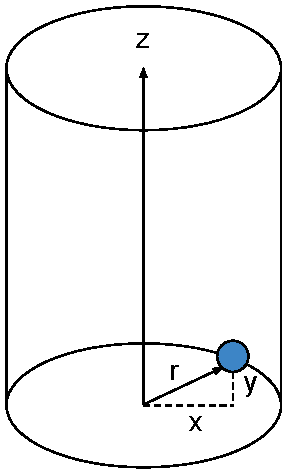
\includegraphics[width=0.2\textwidth]{cartesian_cylinder.pdf}
  \caption{Using the nearest pore center as the origin, we represented the solute's
  location along the pore axis in terms of the $z$ coordinates and their radial distance
  from the pore centers in 2 dimensions, $x$ and $y$.}\label{fig:cartesian_cylinder}
  \end{figure}
  
  \noindent We applied the IHMM to each of the 24 solute trajectories independently.
  \begin{itemize}
    \item Although the IHMM is capable of identifying an infinite number of states, 
    a Dirichlet Process tends to exhibit a ``rich get richer" effect, favoring
    a fewer number of states.
    \item By applying the algorithm to each trajectory independently, we reduce
    the possibility of lumping together multiple similar states which we
    would prefer to stay separated before clustering.
%    \item From a practical implementation standpoint, the algorithm is written
%    such that we must put a cap on the maximum number of states. We chose to 
%    allow up to 100 states for each trajectory although the algorithm typically
%    finds within the range of 5-15 states. 
    % BJC2: There will probably be a figure telling the number of states for 
    % each trajectory.
  \end{itemize}
  
  % BJC5: For the paper, this paragraph and figure might be better suited for the supporting information
  % BJC5: maybe even for the thesis
  \noindent The states identified by the IHMM are heavily influenced by the Gaussian prior
  placed on $\mathbf{c}$ in Equation~\ref{eqn:var}.
  \begin{itemize}
    \item The entries of $A$ and $\Sigma$ do not vary over a wide range, so
    the final parameters were relatively insensitive to the priors.
    \item In order to maximally automate the IHMM procedure, we attempted to
    parameterize the prior on $\mathbf{c}$ in an intelligent way.
    \item The prior parameters should be chosen such that the mean level of 
    each state lies within a region of reasonable probability of the prior (see
    Figure~\ref{fig:prior_guesses}).
    \item In each dimension, we defined the prior mean to lie halfway between the 
    maximum and minimum of each trajectory dimension. 
    \item To parameterize the prior's variance in each dimension, we defined the
    maximum and minimum to be 2 standard deviations from the prior mean.
    \item Although this approach has worked quite well for the data in this work,
    it is important to check the results to determine whether further adjustments
    to the prior might be needed.
    \item In the Supporting Information, we show the result of a parameterization
    where the prior parameters of $c$ were poorly chosen. %TODO
  \end{itemize}
  
  %BJC2: I think it would be useful to continue using this trajectory to illustrate 
  % the parameterization process. It might be bunch of plots stacked on each other.
  %BJC2: More labels would be useful if not cluttered
  \begin{figure}
  \centering
  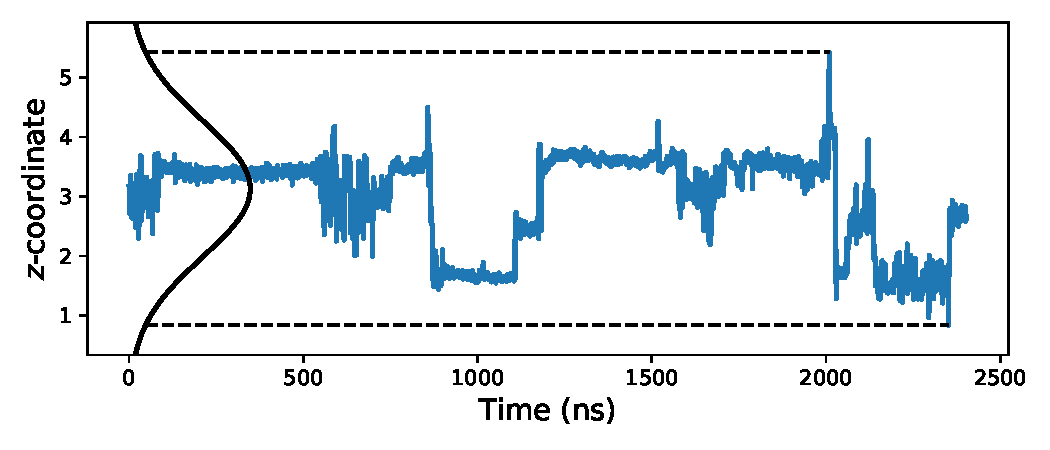
\includegraphics[width=\textwidth]{prior_guesses.pdf}
  \caption{The parameters of the prior on the mean vector, $c$, (black line), which
  represents the coordinates at which solute are trapped, should be chosen such
  that the mean levels of each state identified in the trajectory (blue line) lie within
  regions of the prior with reasonable probability. We chose the mean of the prior 
  as halfway between the maximum and minimum of each trajectory dimension. We chose 
  $\sigma$ of the prior by defining the maximum and minimum to be 2 standard deviations
  from the mean (dashed lines).}\label{fig:prior_guesses}
  \end{figure}
  
  We ran 2000 iterations of the IHMM procedure in order to arrive at converged 
  state sequences and parameters for each state.
  \begin{itemize}  
    %MRS3: can you say more which categories converged quickly?
    %BJC3: I imagine states with less sampling converge slower. But I'll need to
    % look further into this.
   \item Most parameters converged quickly (within 50-100 iterations) while
    others took up to 1000 iterations.
    \item We defined the finalized parameters of each state as the average
    of the parameters from each iteration recorded after the equilibration 
    time point.
    % MRS3: averaged and used this as estimate for running models later? 
    % BJC3: yes, well for clustering. Tried to clarified above
    % MRS3: other possbility is maximum a posteriori estimate, but for peaked 
    % symmetric distributions, it's essentially the same.
    %BJC5: moved following point to earlier in methods.
%    \item We detected equilibration of the parameters using the module 
%    \texttt{pymbar.timeseries.detect\_equilibration} on the time series of 
%    parameter estimates. 
    \item We found the equilibration time point of each component of the 
    $\mathbf{c}$ vector as well as $A$ and $\Sigma$ matrices, and then used the longest
    equilibration time of all dimensions as the equilibration time point.
  \end{itemize}
  
  We reparameterized the time series, preserving the state sequence, in terms
  of the radial and axial coordinates ($r$, $z$) because $x$ and $y$ aren't 
  meaningful alone due to the system's radial symmetry.
  \begin{itemize}
    %MRS4: Do you need to convert the covariance to cylintrical coordinates here before clustereing? 
    %BJC4: No because I only convert the coordinates to cylindrical and then use 
    % the inference part of the IHMM to estimate the covariance.
    \item We converted the $x$ and $y$ center-of-mass coordinates to $r$.
    \item We fixed the state sequence from the 3D parmeterization and applied the
    inference component of the IHMM procedure to the cylindrical trajectories in
    order to estimate the VAR(1) parameters in terms of $r$ and $z$.
  \end{itemize} 
  
  \noindent We clustered like parameter sets in order to reduce the state space to
  a more easily interpretable size.
  \begin{itemize}
  	\item For each solute studied, we identified 200-325 independent states, each
   	with separate VAR(1) parameters.
   	\item Many of these states exhibit very similar dynamical behavior except their
   	mean levels are different.
  \end{itemize}
  
  We reduced the parameter space used agglomerative clustering, a hierarchical
  clustering approach which uses a linkage criteria in order to successively merge
  similar clusters until a desired intracluster distance threshold or number of
  clusters is reached. 
  \begin{itemize}
   	\item We used the Ward linkage criteria, which works to minimize the sum of
   	the squared differences within all clusters.
   	\item We elected to choose the number of clusters rather than the distance
   	threshold.
   	\item For our data, non-parameteric methods such as Bayesian Gaussian mixture
   	models tend to delocalize the clusters in parameter space (see Supporting
   	Information).
   	%BJC: will show Gaussian mixture model which has a cluster engulfing another cluster, so it's tails are on both sides of the center cluster.
  \end{itemize}  
  
  % BJC2: this part may expand a bit if I try different clustering approaches. But
  % this is the one I'm going with for now.
  We clustered based on the two diagonal entries of $A$ and $\Sigma$ as well as the
  radial means, $\mu_r$, for a total of 5 variables.
  \begin{itemize}
   \item One can choose alternative clustering features, such as the eigenvalues of
   the $A$ and $\Sigma$ matrices, but we chose their diagonals because they can be
   easily translated to solute behavior.
   %MRS4: suggest translating them here into solute behavior for the reader!
   \item We also chose to cluster the diagonals of each matrix and the radial means
   independently before combining the clusters to assign final state labels. 
   \item If we divide the total states into $m$ clusters based on the diagonal entries
   of $A$, $n$ more clusters based on the diagonal entries of $\Sigma$, and $k$ clusters
   based on $\mu_r$, then there are a total of $mnk$ possible cluster combinations.
   \item This allows slightly more flexibility in the total number of states compared
   to clustering on all five features at once, since there can be up to, but not 
   necessarily exactly, $mnk$ states. 
   %MRS4: so no clustering based on transition probablity, correct?
   %BJC4: not at the moment. That might have been more helpful if I was first-order differencing.
  \end{itemize} 
  
  Choosing the number of clusters can be somewhat subjective so
  we attempted to add some structure to the selection process by following
  a set of qualitative and quantitative guidelines.
  \begin{itemize}
  	%BJC3: not sure if the commented point worth making.
%    \item We should expect a relatively high number of states. If we only consider
%    the diagonal entries of the $A$ and $\Sigma$ matrices, a total of four independent
%    variables, we can consider clustering each into at least two groups (higher versus
%    lower values), which implies $2^4$ distinct dynamical behaviors. 
    \item We used the silhouette test in order to score the quality of
    clustering as a function of the number of clusters chosen.
    \item For our data, the silhouette test generally favors the lowest number
    of clusters possible (see Supporting Information).
    \item However, choosing too few clusters tends to result in 
    inadequate distinguishment between visually obvious differences in 
    dynamic behavior.
    \item This results in finalized parameter sets that are averages of
    distinct behavior which presents further problems with the predictive
    modeling that we discuss later on.
    \item We aimed to maintain the highest silhouette score, and thus lowest
    number of clusters, possible while verifying that visually distinct 
    states stayed separated.
    \item Based on these guidelines, we decided to group the $A$ and $\Sigma$
    parameters into five clusters each and the radial means into three clusters. 
	\item Of the 75 distinct states allowed by this formulation, the solutes
	in this study clustered into 30--33 distinct clusters.  %BJC5: need to check these numbers
	\item While this may seem like a high number of states, many are sampled
	infrequently.
  \end{itemize}

  \noindent We remapped the state sequence based on the cluster assignments and
  generated a state transition probability matrix, $T$.
  \begin{itemize}
   \item The IHMM algorithm also produces an estimate of $T$, but since we 
   fixed the state sequence, we decided to explicitly calculate $T$ by 
   counting the number of transitions between states compiled across all 
   trajectories.
  \end{itemize}  
  
%  We obtained $\mathbf{c}$ vectors of the clustered states by averaging 
%  each value of $\mathbf{c}$ assigned to the same cluster.
%  \begin{itemize}
%   \item We only care about the $r$ component of $\mathbf{c}$ because solute
%   trajectories are not bound in the $z$ direction.
%  \end{itemize}

  We used the parameter inference component of the IHMM algorithm in order to 
  infer $A$, $\Sigma$ and $\mu_r$ of the clustered states.
  \begin{itemize}
   %BJC2: I'm unsure of the precise reasoning here.
   \item We could not simply take the mean of the clustered 
   $A$ and $\mathbf{e}_t$ parameters because it is not clear that this is a linear 
   operation for this problem. 
   \item To circumvent this problem, we modified the ($r$, $z$) solute
   trajectories so that they had a mean of zero, leaving only the 
   fluctations. 
   \item We did this by subtracting the maximum likelihood estimate
   of the $\mathbf{c}$ vector from each same-state segment of the unclustered
   trajectory.   
   \item We used the IHMM algorithm on this modified trajectory to infer
   the clustered state parameters by fixing the clustered state sequence. 
  \end{itemize}
  
  \noindent Finally, we generated stochastic trajectory realizations using the clustered
  parameter sets.
  \begin{itemize}
    \item We drew state sequences with transition probabilities given by $T$.
    \item While in a given state, we simulated motion according to the VAR(1)
    parameterization of that state.
    \item After each state transition, we reset the unconditional mean of each 
    state based on the particle's position immediately before the state transition
    occurred.
  \end{itemize} 
  
  % BJC5: not sure what to title this. Or break it into more sections.
  \subsection{Calculation of Physical Interactions}\label{method:interactions}
  
  We determined the number of hydrogen bonds between each solute and the membrane
  as a function of time.
  \begin{itemize}
    \item Based on the geometric criteria of Luzar and Chandler, we define a hydrogen
    bond to exist if the distance between donor, D, and acceptor, A, atoms is less 
    than 3.5\AA~and the angle formed by $D-H \cdots A$ is less than 30
    $\degree$.~\cite{luzar_effect_1996}
  \end{itemize}
  
  We estimated the lifetime of hydrogen bonds by recording the length of 
  sequential frames where solute remained hydrogen bonded.
  \begin{itemize}
    \item We still counted sequences where hydrogen bonds were broken for
    a single frame before reforming.
    \item We reported the 95th percentile of hydrogen bond lifetimes.
  \end{itemize}
  
  We also measured the degree of association between solutes and sodium ions on a
  frame-by-frame basis.
  \begin{itemize}
    \item We define a sodium ion to be associated with an atom if they are within 
    2.5 \AA~of each other, as determined in our previous work.~\cite{coscia_chemically_2019}
  \end{itemize}
  
  We developed a way to measure the local density of the membrane at arbitrary
  points in the unit cell.
  \begin{itemize}
    \item We histogrammed the positions in three dimensions
    \item Since our system is in a monoclinic unit cell, we periodically replicated
    the system in +/- x, y and z direction and then set the bounds on the
    histogram to create a rectanglular box encompassing the unitcell with a 1 nm
    buffer between the histogram unitcell boundaries.
    \item We then used a regular grid interpolator in order to allow interpolation
    at arbitray points within the grid.
  \end{itemize}
  
  We quantified average solute movement using the time averaged mean squared 
  displacment (MSD) of the solute center of mass trajectories.
  \begin{itemize}
  
 	\item The time-averaged MSD measures all observed displacements over time lag $\tau$:
  	\begin{equation}
  	\overline{z^2(\tau)} = \dfrac{1}{T - \tau}\int_{0}^{T - \tau} (z(t + \tau) - z(t))^2 dt
  	\label{eqn:tamsd}
  	\end{equation}
  	where T is the length of the trajectory.
  	\item We reported 1$\sigma$ confidence intervals based on the results of 200 
  	bootstrap trials where calculated the mean of $n$ randomly chosen trajectories 
  	with replacement from the pool of trajectories, where $n$ is the number of trajectories.
  \end{itemize}

  
  \subsection{Estimating Flux and Selectivity}
  %BJC: can make this discussion somewhat short since it's already in previous paper. 
  %MRS4: yes, can be short
  % Should probably just hit all the main equations quickly.
  
  \noindent We calculate first passage times by propagating stochastic trajectories until they
  reach distance $L$. \\
  
  We determine the mean first passage time (MFPT) using the following equation:~\cite{cussler_diffusion:_2009}
  \begin{equation}
  P(t) = -\frac{1}{\sqrt{\pi}}e^{-(L - vt)^2 / (4Dt)}\bigg(-\frac{D(L - vt)}{4(Dt)^{3/2}} - \frac{v}{2\sqrt{Dt}}\bigg)
  \label{eqn:passage_times}
  \end{equation}
  
  \noindent Flux, $J$, is simply 1 / MFPT by the Hill relation.~\cite{hill_free_1989} \\
  
  In our previous work, we showed that, in the absence of convective solute flux, selectivity
  towards solute $i$ versus solute $j$ can be calculated by:  
  \begin{equation}
  S_{ij} = \frac{J_i / \Delta C_i}{J_j / \Delta C_j}
  \label{eqn:selectivity}
  \end{equation}
  where $\Delta C_j$ is the trans-membrane concentration difference.

  \section{Results and Discussion}
  
  Solutes in this system show a wide range of behavior influenced by the 
  heterogeneity of the membrane's nanostructure as well as the interactions 
  between monomer and solute chemical functionality. 
  \begin{itemize}  
  	\item Our application of the IHMM does a good job of identifying and
  	distinguishing these behaviors.   	
  	\item The following approach to analysis demonstrates how one can discover and explain the very complex behavior exhibited by solutes over long MD trajectories 
   in terms of solute-membrane interactions.
%  	\item Clustering the behaviors helps us to tell a coherent story which
%  	emphasizes those interactions which most heavily influence solute transport.
	\item Further, we can use the IHMM in order to generate stochastic trajectories,
	with dynamics similar to MD, so that we can estimate macroscopic transport
	properties.
  \end{itemize}  	

  \subsection{Automatic Detection of Distinct Dynamical Modes}\label{section:find_modes}
  
  %BJC3: I'm not sure if it's worth talking about all of the solutes in this section.
  % there is a lot to talk about just with methanol (which is all I've done for now -- wanted to
  % get feedback on analysis approach).
  %BJC3: I see this more as a demonstration of the model. I think this work has higher
  % impact potential so I don't want it to be 15 pages.
  %BJC3: Although, it might be a good idea to include Urea or Acetic acid as a second example
  % molecule because their behavior is pretty different since their carbonyl group tend to 
  %MRS4: there should be SOME summary information on the other molecules, but it can just be the conclusions.
  % associate with sodium a lot.
  
  We applied the IHMM to all trajectories of each of the four solutes studied.
  \begin{itemize}
    \item Based on our choice of clustering, we identified over 30 distinct dynamical
    modes for each solute.
    \item Many of these modes are sampled very infrequently and thus do not merit significant study.
    \item In this section, we explore a subset of this data, focusing on the states
    and dominant interactions most common to solute trajectories. 
  \end{itemize}  
  
  \noindent Methanol exhbits a range of dynamic behavior.
  \begin{itemize}
    \item In Figure~\ref{fig:mechanism_map}, we plot a representative 2D methanol 
    trajectory in cylindrical coordinates.
    \item The coordinates are colored according to the cluster with which methanol's
    dynamics are most consistent, which implies that this particular methanol 
    trajectory exhibits 8 distinct dynamical behaviors (in order of their first appearance,
    they are colored dark yellow, red, light blue, light green, orange, blue, teal and lime green). 
    \item The solute timeseries are coupled with color coded bars which describe the
    solute's local environment and physical interactions that it undergoes at that
    trajectory frame.
    \item From the top, they describe whether the solute is associated with sodium,
    whether the solute is hydrogen bonding with the monomer as well as to what part of
    the monomer it is hydrogen bonding, and finally, the local number density 
    surrounding the solute. 
    %and the radial location of the solute with respect to the nearest pore
    %center (this information is redundant but can be a useful visual aid).
  \end{itemize}
  
  \begin{figure}
  \centering
  \begin{subfigure}{0.75\textwidth}
  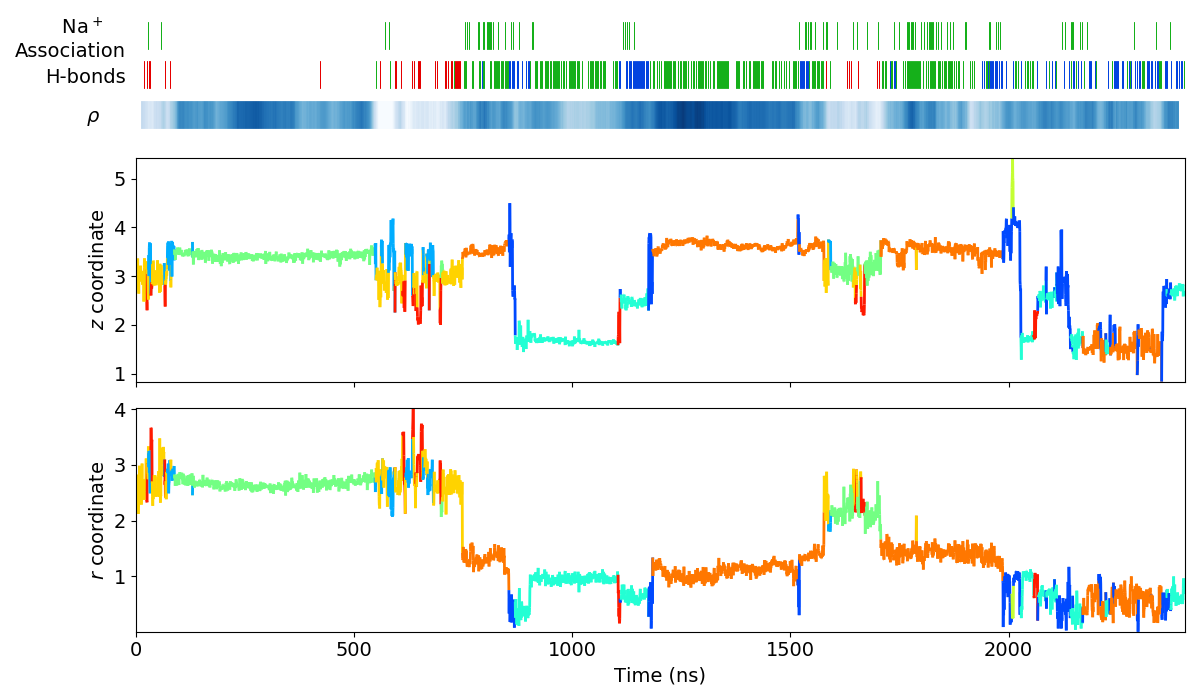
\includegraphics[width=\textwidth]{mechanism_map.png}
  \caption{}
  \end{subfigure}
  \begin{subfigure}{0.24\textwidth}
  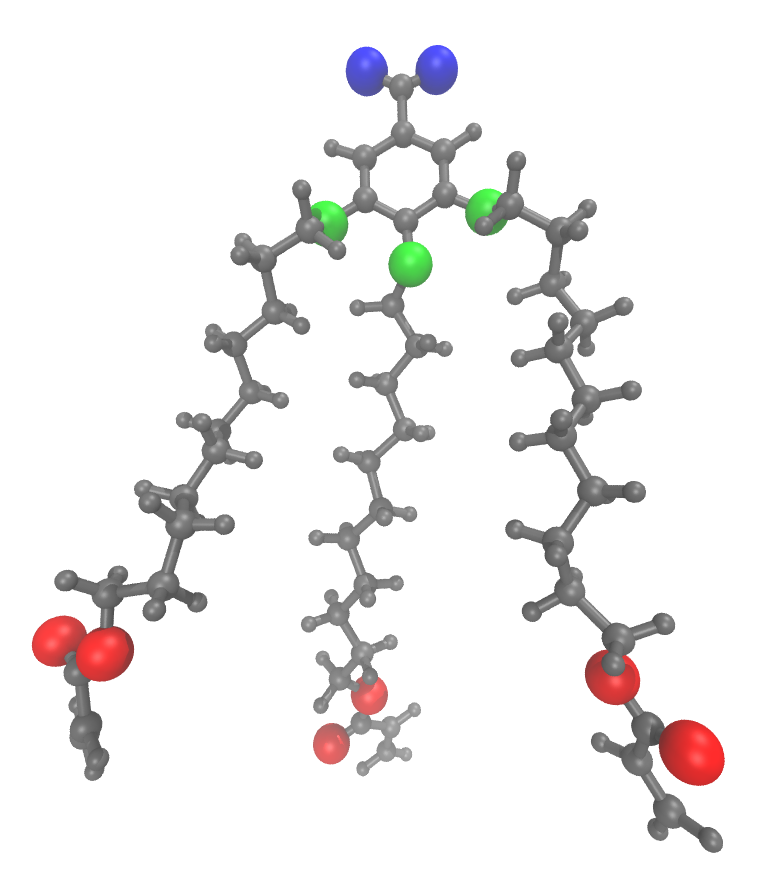
\includegraphics[width=\textwidth]{monomer_oxygens.png}
  \caption{}
  \end{subfigure}
  \caption{(a) We can learn a significant amount of detail about solute motion by viewing 
  solute trajectories color-coded according to their clustered dynamical behavior alongside
  plots of the dominant molecular interactions and descriptions of the membrane's local 
  environment. In the plot above, we show the radial and axial coordinates of a single
  methanol molecule over the course of the equilibrated portion of its MD simulation.
  Disjoint segments of the same color imply the solute behaves similarly at different 
  points of the trajectory because their VAR parameters place them in the same cluster. 
  There are eight distinct dynamical modes exhibited by this trajectory. In order
  of their first appearance, they are colored dark yellow, red, light blue, light green,
  orange, blue, teal and lime green. On the top of the plot are bars which represent different
  physical interactions and the membrane's local environment as a function of time. The top 
  bar is colored green at time points where solutes are associated with sodium. Methanol 
  associates with sodium ions relatively infrequently. The next bar down is colored when hydrogen
  bonds exist. The colors match the enlarged oxygen atoms highlighted in (b). Blue slivers
  correspond to hydrogen bonds donated to the monomer's carboxylate head group. Green slivers
  corrrespond to  hydrogen bonds donated to the ether linkages between the head groups
  and tails. Red slivers correspond to hydrogen bonds donated to the oxygens on the ends
  of the monomer tails. Methanol exhibits significant hydrogen bonding with all parts of
  the monomer. Which part of the monomer methanol hydrogen bonds to is heavily correlated
  to the solute's $r$ coordinate. Finally, the bar with the blue gradient represents the local 
  membrane density based on the solute's ($r$, $z$) coordinate. Darker shades of blue
  correspond to higher membrane densities. The density appears to be higher when methanol
  motion is restricted (e.g. from 75 to 550 ns). It is relatively low in areas where methanol's
  position fluctuates significantly (e.g. from 550 to 700 ns). 
  %Finally, the bottom bar
  %simply color-codes the solute's radial distance from the pore center. This information
  %is the same as shown by the radial coordinate but can be a helpful visual aid when
  %studying the other bars.
  }\label{fig:mechanism_map}
  \end{figure}

  \noindent One can gain useful chemical intuition just by studying plots like
  Figure~\ref{fig:mechanism_map}.
  \begin{itemize}
    \item It is clear that, for methanol, association with sodium is a much rarer
    interaction than hydrogen bonding with the LLC monomers.
    \item Methanol hydrogen bonds to all regions of the monomers dependent on
    its radial position.
    \item Its fluctuations tend to be smallest when hydrogen bonded or in areas
    of high local number density. 
    \item For example, from approximately 75 to 525 ns, methanol appears to be trapped
    in a high density region of the tails.
    \item In the time that follows, it enters a region of relatively low density
    where fluctuations are quite large. 
    \item During this time period, there is intermittent, short-lived hydrogen 
    bonding with the oxygen atoms at the tail ends, as suggested by the frequent 
    state changes during that time period and red slivers in the bar above.
    \item Signficant hops in the $z$ direction appear to be described by the dark blue
    state.
    \item After entering the dark blue state ca. 850 ns, methanol appears to jump
    signficantly in the $z$ direction from a hydrogen bonded state with the ether 
    linkages to a hydrogen bonded state with a head group in a monomer below it.
  \end{itemize}

  %BJC3: I think I'll just skip to the clustered results. I'd like to keep this
  % paper on the shorter side.
%  The IHMM does a sufficient job of capturing differences in solute dynamics
%  for individual trajectories.
%  \begin{itemize}
%    \item In Figure TBD, we show the states identified by the IHMM for a single
%    methanol trajectory. The IHMM found x number of states.
%  \end{itemize}
  
%  Depending on the path followed, solute trajectories show diverse behavior.
%  \begin{itemize}
%    \item Some show lots of movement
%    \item Some show almost no movement
%    \item While all trajectories might not be the same, it is likely that 
%    multiple trajectories might share some similar behavior.
%  \end{itemize}

  \noindent It is clear that there is a wealth of information in these plots, but they don't give the complete picture needed in order to formulate LLC membrane design principles.
  \begin{itemize}
    \item One can analyze each segment sequentially and form a clear picture
    of this instance of methanol's behavior without the need to visulize
    the traejectory with software like VMD.
    \item However, it is still possible to gain a more general understanding of methanol's average behavior.
  \end{itemize}
  
  %BJC: I'm not sure whether to spell out the numbers or not. 'six state' versus '6 states'; 'eight out of 24' or '8 out of 24'
  % 'State one or State 1' 
  \noindent We may learn the most by studying the dynamical modes common to the majority of 
  the solute trajectories.
  \begin{itemize}
    \item Using the IHMM, we identified 33 total dynamical modes exhibited by 
    methanol. 
    \item Of those, only six states appear in a third (8 out of 24) or more methanol 
    trajectories, and three of them appear in over 50 \% of the methanol trajectories.
    \item 12 of the detected states are shared by two or less methanol trajectories.  % 23 in 3 or less -- not sure which is better to say
    \item In Figure~\ref{fig:common_states_MET_lines}, we plot representative dynamics
    of each of the six states which we determined to be prevalent.
    \item We also chose to study a seventh state, which only appears in three out of
    24 trajectories, because methanol experiences very long periods of entrapment
    while in this state. Long trapping events, even if they are relatively rare, will
    have a significant influence on solute flux.
    \item No trajectory contains all seven states. However, the trajectory in 
    Figure~\ref{fig:mechanism_map} exhibits all modes except states 6 and 7.
    \item The states in Figure~\ref{fig:common_states_MET} are colored to match
    states that also appear in Figure~\ref{fig:mechanism_map}.
  \end{itemize}
    
  \noindent We can begin to dissect the dynamics of each state by studying their parameters.
  \begin{itemize}
    \item States 1, 3 and 5 have radial means near 1 nm or less (see y axis of $r$ direction plot in
    Figure~\ref{fig:common_states_MET_lines}), which suggest that they occur
    close to the pore centers. 
    \item States 2, 4, 6 and 7 occur well within the tail region of the membrane.
    \item States 1 and 2 have higher covariances in both the axial and radial
    directions compared to all other states.
    \item Covariance in each dimension appears to have a strong correlation.
    \item States 3 and 5 (in the pore region) as well as states 4, 6 and 7 (in the tail region) are primarily distinguished based
    on their autoregressive coefficients, A. 
    \item Higher values of A generally lead to more wandering about the state mean.
    \item One could argue that the parameters of states 3--7 are actually very close which
    suggests that solutes might behave alike in topologically distinct regions of the 
    membrane.
  \end{itemize}

  Despite some similarity in their VAR parameters, the length of time spent in states 3--7 
  appears to be dependent on the solute's radial location.
  \begin{itemize}
    \item Based on the self-transition probabilities, we estimated the average time
    spent by each solute in each state (Figure~\ref{fig:dwell_times_MET}).
    \item States 3, 5 and 7 have long dwell times relative to the rest because
    they have high self-transition probabilities.
    \item Somewhat surprisingly, both states 3 and 5 correspond to solutes located close to
    a pore center, where one might expect solute motion to be less restricted.
    \item Although solutes in states 4 and 6 are in the viscous tail region, their
    dwell times are only intermediate. This could be due to imhomogeneity in the
    tail region which causes transitions between many different trapped states but
    with litle net effect on solute MSD. 
    \item However, there are instances of states within the tail region with dwell 
    times that exceed 100--200 ns, as shown by our inclusion of state 7.
%    \item These long dwell times have a significant effect on dynamics and are
%    worth studying.
    \item There are no other states with dwell times longer than state 5 in the pore 
    region.
  \end{itemize} 
  
  \noindent States 1 and 2 exhibit the shortest dwell times of the states studied.
  \begin{itemize}
      \item This is consistent with the trajectory in Figure~\ref{fig:mechanism_map}.
      \item State 2 is the shortest lived state, appearing to bridge other tail region
      states. 
      \item State 1 appears to represent a significant hopping state. 
      \item It has a high covariance and occurs near the pore center, where there is
      less obstruction to solute motion.
      \item It's dwell time of ca.~8 ns, suggests that solutes stay in this highly
      mobile state for long enough for their positions to displace signficantly.
  \end{itemize}
  
  \begin{figure}
  \centering
  \begin{subfigure}{0.6\textwidth}
  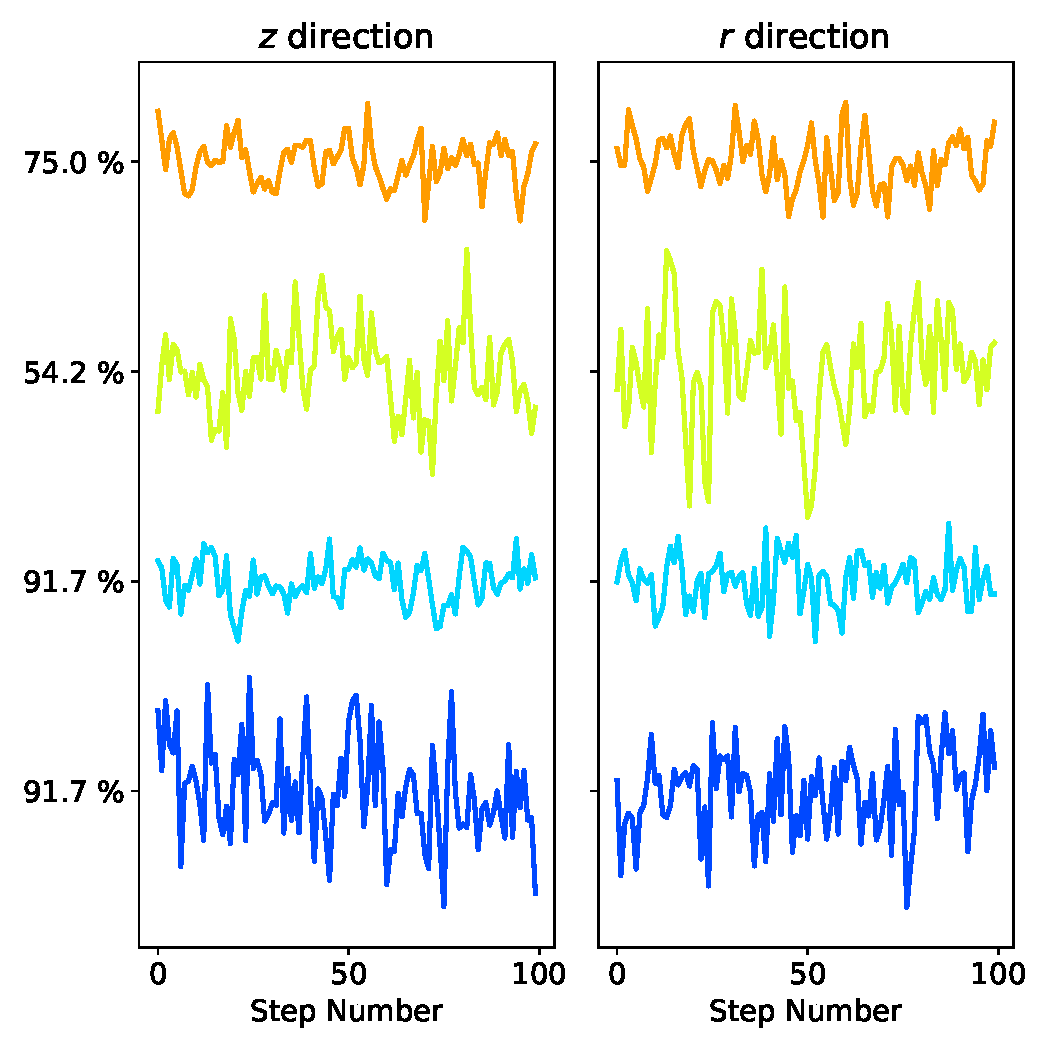
\includegraphics[width=\textwidth]{common_states_MET.pdf}
  \caption{}\label{fig:common_states_MET_lines}
  \end{subfigure}
  \begin{subfigure}{0.35\textwidth}
  % BJC: I'll bootstrap some errorbars on this by drawing the transition probabilities 
  % from a dirichlet distribution.
  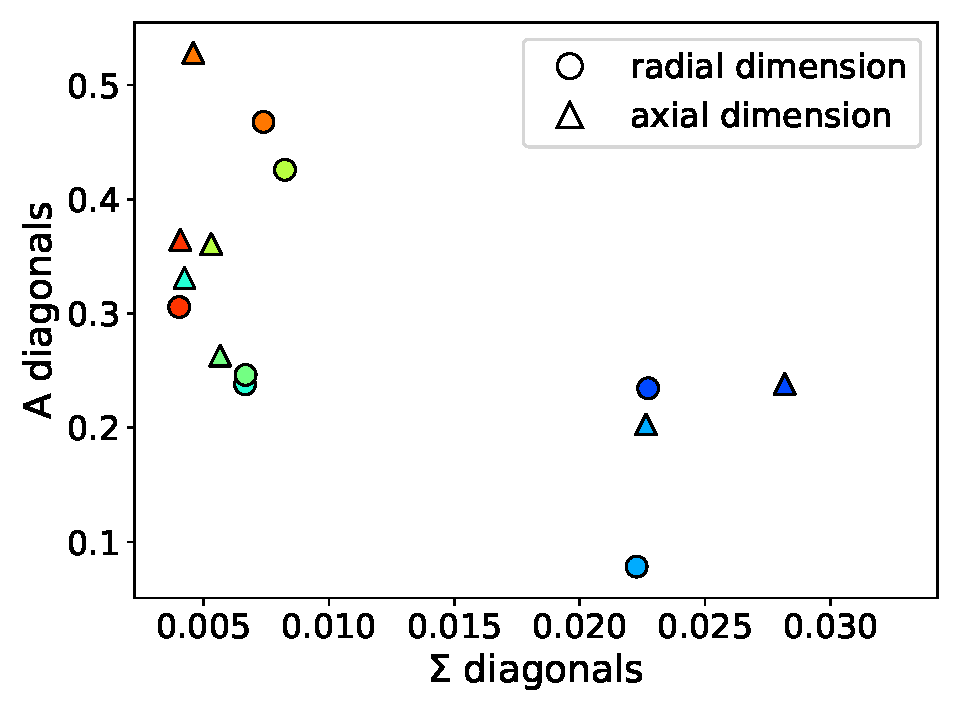
\includegraphics[width=\textwidth]{A_sigma_scatter_MET.pdf}
  \caption{}\label{fig:A_sigma_scatter_MET}
  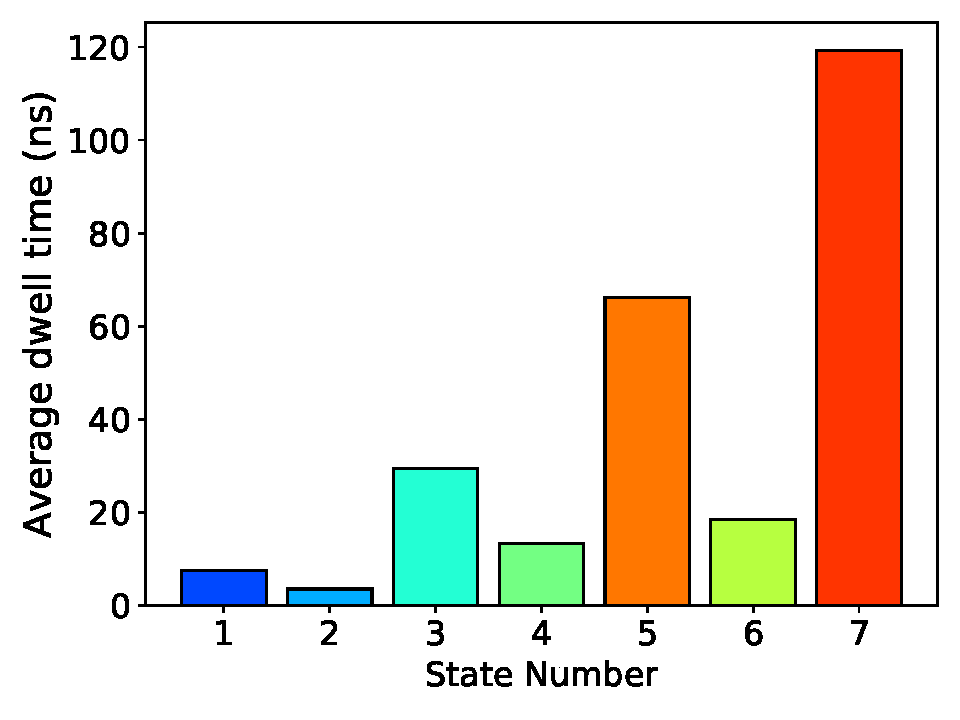
\includegraphics[width=\textwidth]{dwell_times_MET.pdf}  %BJC5: maybe better as 95 % confidence rather than mean
  \caption{}\label{fig:dwell_times_MET}
  \end{subfigure}
  \caption{We can learn the most about methanol's behavior by studying the dynamics
  of the states common to many of the methanol trajectories. In (a), we show representative
  dynamics of six states that are common to more than one third of the solute trajectories. 
  The $y$-axis labels of the $r$ coordinate plot specify the radial mean of each clustered 
  state. The percentage of trajectories in which the states appear are labeled to the right of
  the $r$ plots. States 1--5 appear in the trajectory shown in Figure~\ref{fig:mechanism_map}
  and are colored to match for easy visual comparison. All time series have a mean of zero and are
  shifted to put the mean in line with the $y$-axis labels for the purpose of visualizing them. 
  (b) We can begin to understand the solute behaviors demonstrated in (a) by understanding their VAR 
  parameters. States 1 and 2 have higher covariances in both the axial and radial directions compared
  to all other states. This should lead to signficant solute displacement. Covariance in each dimension
  appears to have a strong correlation. States 3--6 all have relatively low covariances, which may
  be characteristic of trapped states. They are primarily distinguished based on the magnitude of their 
  autoregressive coefficients, A, and radial means. Higher values of A imply motion which wanders 
  more about the mean. States 1, 3 and 5 have radial means near 1 nm or less, which suggest that they
  occur close to the pore centers. States 2, 4 and 6 occur well within the tail region of the membrane.
  (c) Using the transition probabilities (p), we estimated the average time spent within each 
  of the states using 1000 simulations of a Bernoulli process where we continued to draw until transitioning
  out of the state with probability 1 - p. Of the prevalent states, states 1 and 
  2 exhbit the shortest dwell times alongside their high covariances. States 5 and 7 have the longest dwell times in the pore and tail regions respectively.
  }\label{fig:common_states_MET}
  \end{figure}
  
  Most of what we have learned thus far has been based on the parameters of our
  model with some qualitative validation using a single methanol trajectory.
  \begin{itemize}
    \item While we may be able to further corroborate our arguments by analyzing more
    individual trajectories, it is more useful to correlate the state behavior with
    solute-membrane interactions.
  \end{itemize}   

  \noindent The types of hydrogen bonding undergone by solutes is dependent on radial
  location (see Figure~\ref{fig:hbond_pichart}).
  \begin{itemize}
    \item States with radial means near 1 nm or less (states 1, 3 and 5) typcially
    hydrogen bond with the monomer carboxylate groups and ether linkages.
    \item States with radial means greater than 1 nm (states 2, 4, 6 and 7) tend 
    to hydrogen bond with the monomer tails.
    \item In the past we've shown that there is a gradual transition from the
  	hydrophilic to hydrophobic region in these membranes, meaning the monomer
  	location is not tightly bound in $r$.
  	\item Therefore, there are instances of hydrogen bond interactions that one
  	might consider uncharacteristic based on the state's radial mean.
  \end{itemize}  
  
  \noindent States which exhibit longer dwell times have longer hydrogen bond lifetimes (see
  Figure~\ref{fig:hbond_pichart}).
  \begin{itemize}
    \item States 3--7 have significantly longer hydrogen bond lifetimes than states
    1 and 2. 
    \item It makes physical and mathematical sense that states 1 and 2 should not 
    stay trapped by hydrogen bonding for long periods because they typically take large
    hops as communicated by their large covariances.
    \item In the tail states, hydrogen bond lifetimes appear to increase with 
    their dwell times.
    \item However, in the pores, the same linear relationship does not hold.
    \item For example, state 5 has the lowest hydrogen bond lifetime of states 3--7
    despite having the second longest dwell times. 
  \end{itemize}
  
  \noindent The local density experienced by solutes may have an impact on the length of solute 
  entrapment.
  \begin{itemize}
    \item On average, solutes in state 5 are surrounded by a relatively high density
    of particles.
    \item Based on its radial location and preference towards hydrogen bonding
    with the ether linkages (see Figure~\ref{fig:hbond_pi_charts}), it is 
    reasonable to assume that while in state 5, methanol spends most of its time just
    outside the pore region, sandwiched between the monomer head groups. 
    \item Although state 5 hydrogen bonds break more frequently than one might expect for 
    a state with long dwell times, it is possible that the solute's dense surroundings
    prevent it from wandering off before the hydrogen bonding interaction can be
    recovered.
    \item This may explain the behavior of methanol in state 5 of the trajectory in
    Figure~\ref{fig:mechanism_map} where the solute's center of mass appears to move
    more freely about its mean than other trapped states.
    \item The data suggests that methanol molecules in state 3 lie closer to the pore
    center than state 5 because they tend to hydrogen bond most frequently with 
    the carboxylate groups.
    \item Methanol molecules which experience state 3 are subject to a lower density 
    local environment and rely more heavily on hydrogen bonding interactions, 
    evidenced by their longer lifetimes, to stay trapped.
  \end{itemize}
  
  States describing behavior in the tail region show a direct relationship between 
  hydrogen bond lifetimes and local density.
  \begin{itemize}
    \item Methanol molecules which experience state 2 spend their time in a low density 
    region of the tails where they can easily break free of hydrogen bonds.
%    \item Methanol molecules in states 4 and 6 experience intermediate-length dwell times.
    \item Conversely, methanol molecules trapped in state 7 are in the densest region of all
    states studied. It is likely difficult for methanol to esacpe these high density regions
    and its position is further stabilized via hydrogen bonding.
  \end{itemize}
  
  %BJC4: I didn't put sodium ion assocaition in this figure because it's infrequent. 
  %BJC4: If I compare to acetic acid or urea, I could add it back. I was thinking of splitting
  % the pi chart in half with slices corresponding to hbonds on one side and association on the other
  \begin{figure}
  \centering
  \begin{subfigure}{0.54\textwidth}
  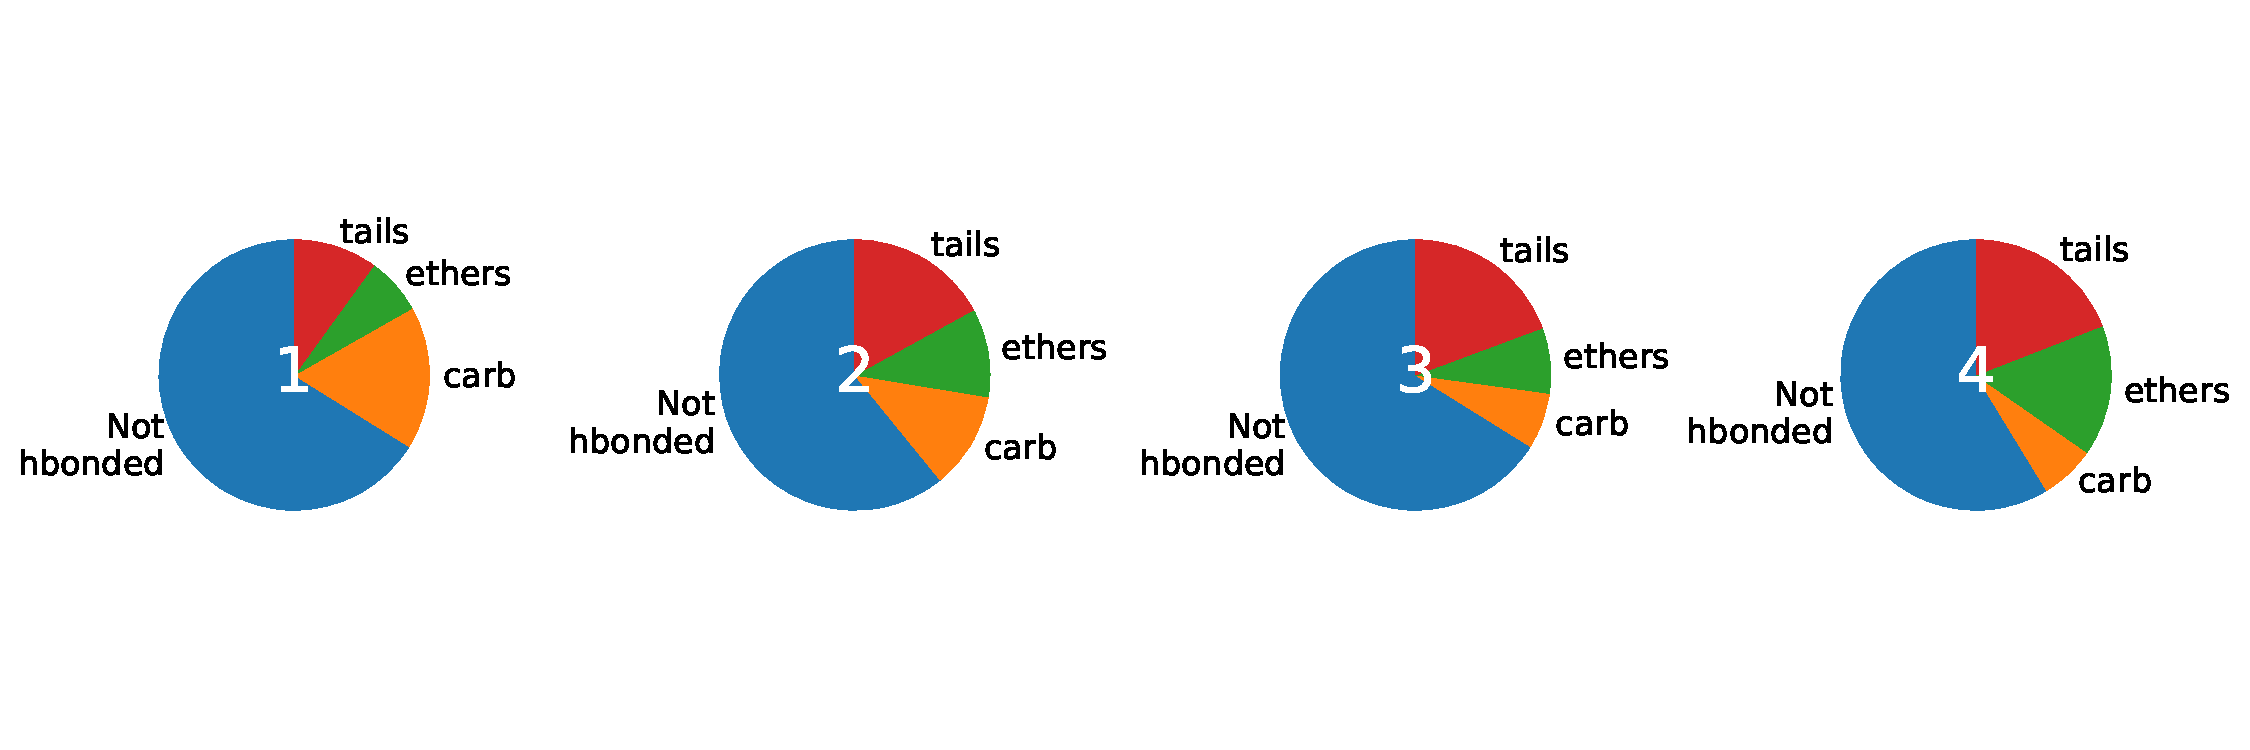
\includegraphics[width=\textwidth]{hbond_pi_charts.pdf}
  \caption{}\label{fig:hbond_pi_charts}
  \end{subfigure}
  \begin{subfigure}{0.45\textwidth}
  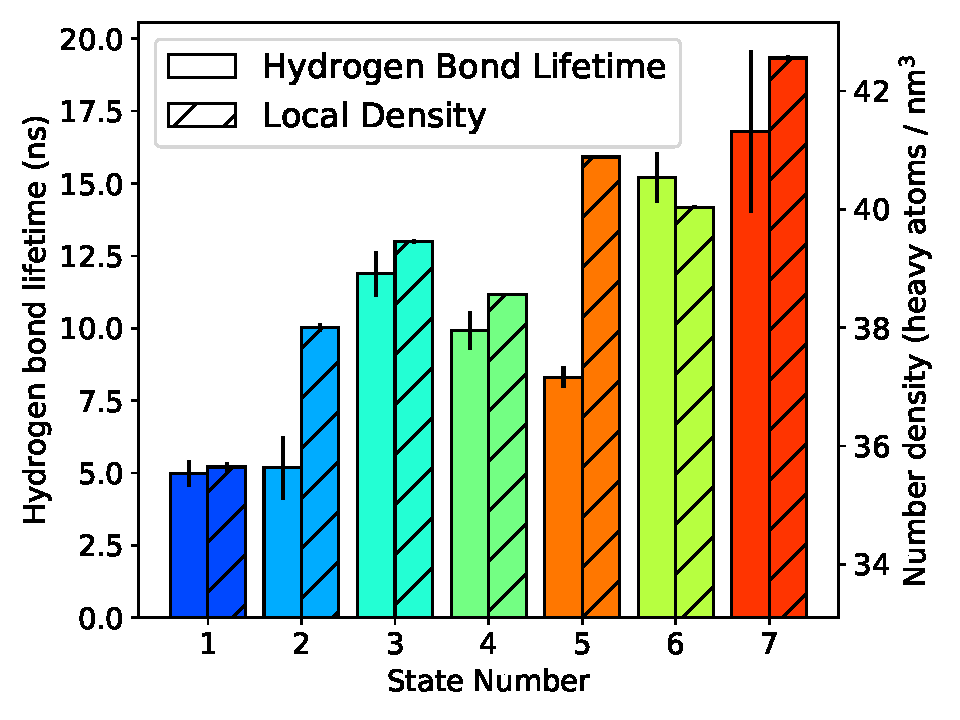
\includegraphics[width=\textwidth]{hbond_lifetimes_density_MET.pdf}
  \caption{}\label{fig:hbond_lifetimes_density_MET}
  \end{subfigure}
  \caption{(a) Methanol hydrogen bonds with different segements of the LLC monomer
  dependent on the state. States with mean radial locations in the pore region tend to
  hydrogen bond with the head groups and ether linkages. States with mean radial
  locations in the tails tend to hydrogen bond with the tail oxygen atoms.
  (b) Hydrogen bond lifetimes and the local density experienced by methanol
  molecules can help us to understand dynamical states in terms of membrane 
  interactions. States 1 and 2, which have large covariances, also have short
  hydrogen bond lifetimes and exist in relatively low density regions. The
  hydrogen bond lifetimes of methanol in states with radial means in the tail
  region tend to increase with local density and mean dwell times. This monotonic
  relationship does not exist for states in the pore region. The high 
  local density experienced by state 5 methanol molecules may explain why 
  hydrogen bond lifetimes are short but dwell times are high. State 5 methanol's
  preference towards hydrogen bonds with ether linkages suggests that the solute
  sits between LLC monomer head group which prevent it from wandering to far
  before recovering its previous hydrogen bond.
  }\label{fig:hbond_pichart}
  \end{figure}
  
  % BJC5: I think I want to do an abbreviated study here on acetic acid or urea 
  % since it will incorporate sodium ion association. 
    
  \subsection{Reproducing MD Trajectories and MSDs with the IHMM}
  
  %BJC5: something we can do for the supporting information to show that this approach is valid: Eliminate nonidealities in our MD trajectories (compared to a pure VAR process) and use toy data to generate trajectories based on some number of states with different parameters. Generate an MSD with those. See if we can reproduce with our model. Can also use this to test new strategies.
  
  We can use the IHMM in order to generate stochastic trajectory realizations
  which bear some qualitatively similar characteristics to those output
  by our MD simulations.
  \begin{itemize}
    \item Because we clustered the data, we are left with a single transition
    probability matrix which allows transitions between dynamical behaviors
    shared by the 24 MD trajectories.
    \item In Figure~\ref{fig:trajectory_realizations_MET}, we show some stochastic
    realizations generated by our models compared directly to MD.
    \item The trajectories show clear periods of entrapment with intermittent hops.
  \end{itemize}
  
  %BJC5: the goal is to figure out how to fix this for the paper.
  %BJC5: this is more of a 'how can this be improved' section for the dissertation.
  The MD trajectories show much broader variability in their overall motion than realizations
  of the IHMM model. 
  \begin{itemize}
  		\item Some trajectories span a wide range of $z$ coordinates, while others stay
  		trapped for nearly the entire simulation.
  		\item Our model is very unlikely to generate trajectories with dwell times similar to 
  		the third MD trajectory shown in Figure~\ref{fig:trajectory_realizations_MET}.
        \item This is because the realizations generated by our model are representative
        of the average behavior of solutes studied.
        \item It is possible that certain states with long dwell times should have been
        clustered as their own, but the transition probabilities would have high uncertainties.
        \item It is also possible that we should not be using a static transition matrix in 
        order to generate stochastic trajectories, but rather sample the rows of the transition
        matrix from a Dirichlet distribution since average dwell times are highly sensitive to
        self transition probabilities.
  \end{itemize}
  %BJC5: maybe a figure showing the MSDs of all the MD trajectories versus a subset of 
  % stochastically generated trajectories. I image the stochastic ones will have a much
  % tighter distribution.

  \begin{figure}
  \centering
  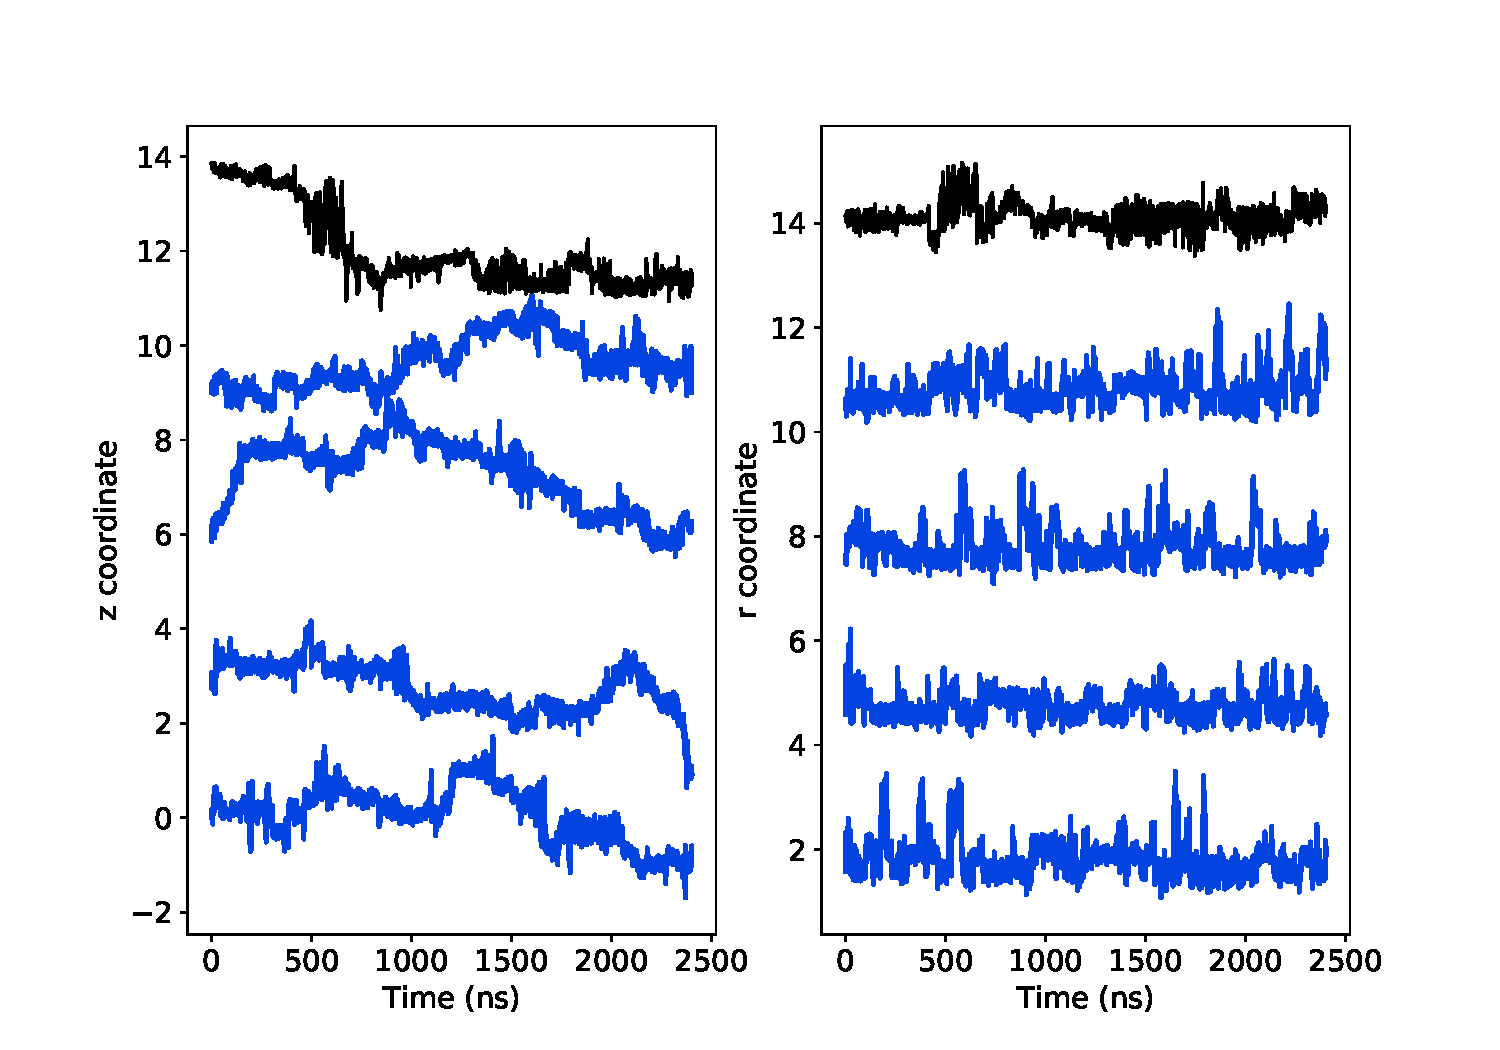
\includegraphics[width=\textwidth]{trajectory_realizations_MET.pdf}
  %MRS5: maybe it would be good to put a dotted line through each of the centers of the offset trajectories?
  %BJC5: TODO 
  \caption{We can generate trajectories which bear some qualitative resemblence to the MD 
  trajectories. Solute trajectories generated by our model (blue) show the same
  hopping and trapping behavior exhibited by MD (black). The behavior of individual 
  MD trajectories tend to show wider variability than our model's realization because
  the model effectively represents the average behavior of the MD trajectories. This 
  implies that much longer simulations or a different method of trajectory generation might
  be necessary in order to obtain stochastic realizations with the same range of behavior
  as MD.
   }\label{fig:trajectory_realizations_MET}
  \end{figure}
  
  \noindent The MSDs calculated by stochastic realizations of our model are
  quantitatively similar to MD.
  \begin{itemize}
  	\item For all solutes except acetic acid, our predicted MSD curve lie close to
  	but below the 1$\sigma$ confidence intervals of MD.
  	\item However, in these cases, the average MD MSDs are driven up by single trajectories
    with uncharacteristically large MSDs.
    \item It is possible that an improved trajectory generation approach may allow
    for this highly variable behavior.
    \item If we remove these uncharacteristic trajectories, the agreement between 
    MD and our realizations improves. 
    \item Acetic acid has no obvious outliers and shows good agreement between MD and
    IHMM realizations.
  \end{itemize}
  
  \begin{figure}
  \centering
  \begin{subfigure}{0.45\textwidth}
  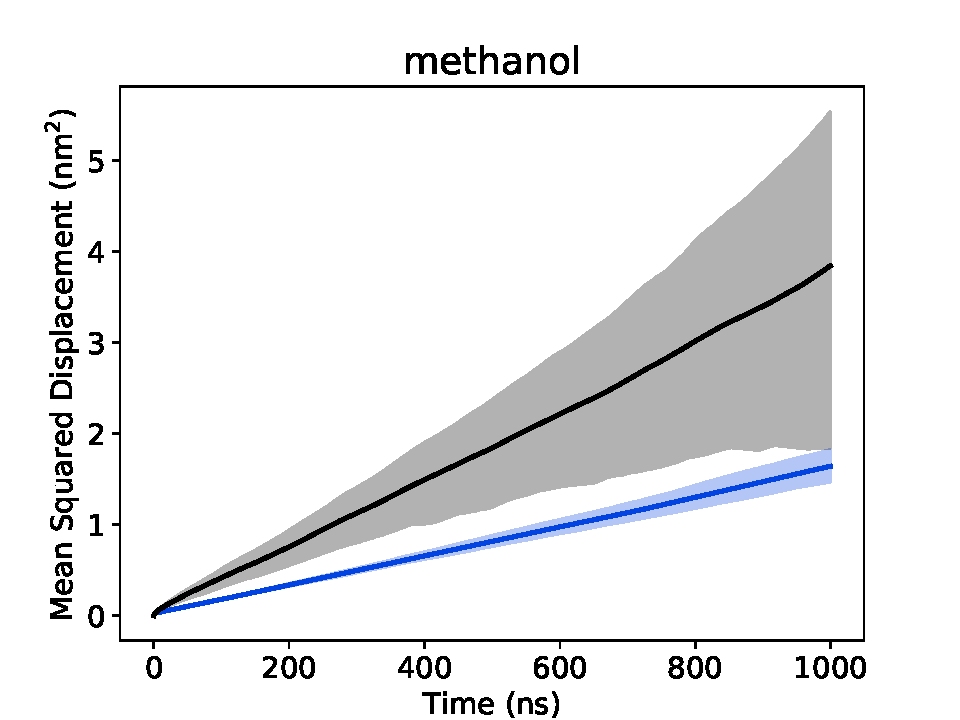
\includegraphics[width=\textwidth]{msd_MET.pdf}
  \caption{}\label{fig:msd_MET}
  \end{subfigure}
  \begin{subfigure}{0.45\textwidth}
  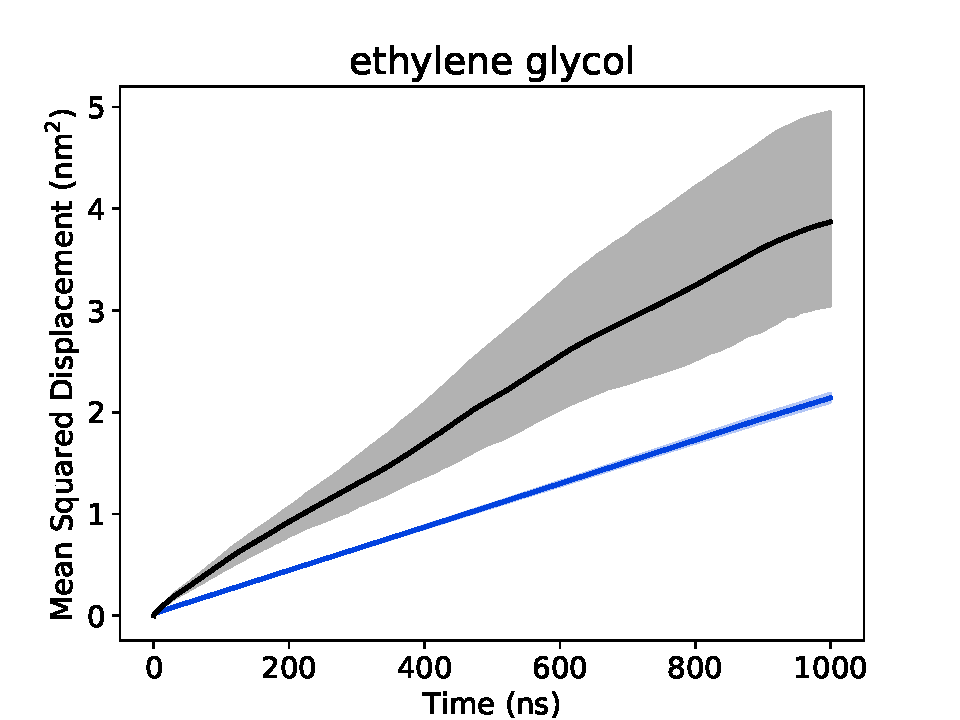
\includegraphics[width=\textwidth]{msd_GCL.pdf}
  \caption{}\label{fig:msd_GCL}
  \end{subfigure}
  \begin{subfigure}{0.45\textwidth}
  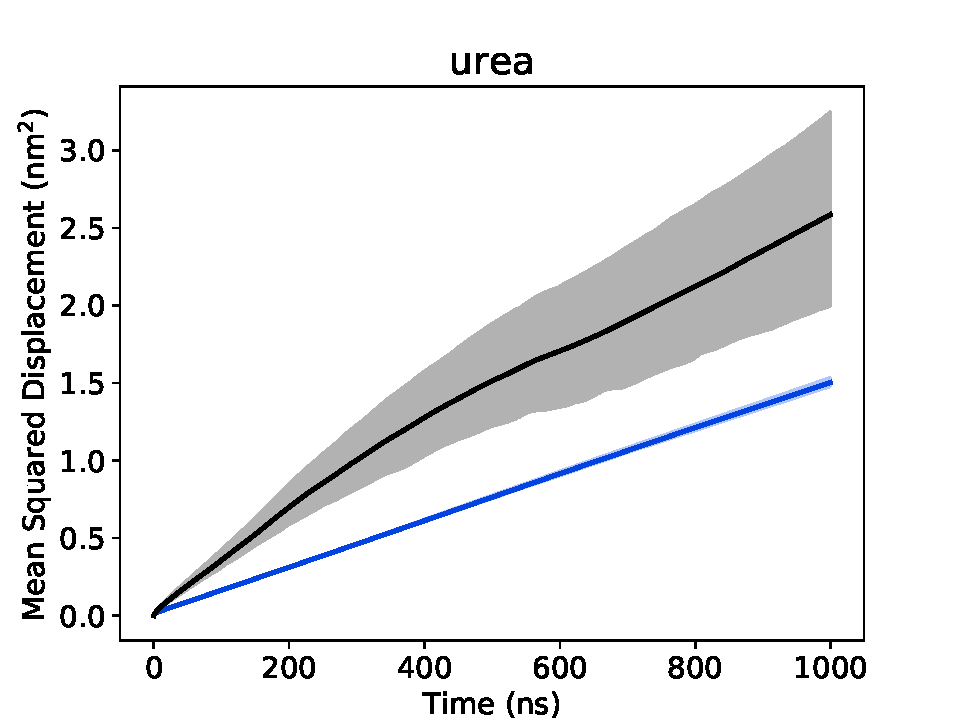
\includegraphics[width=\textwidth]{msd_URE.pdf}
  \caption{}\label{fig:msd_URE}
  \end{subfigure}
  \begin{subfigure}{0.45\textwidth}
  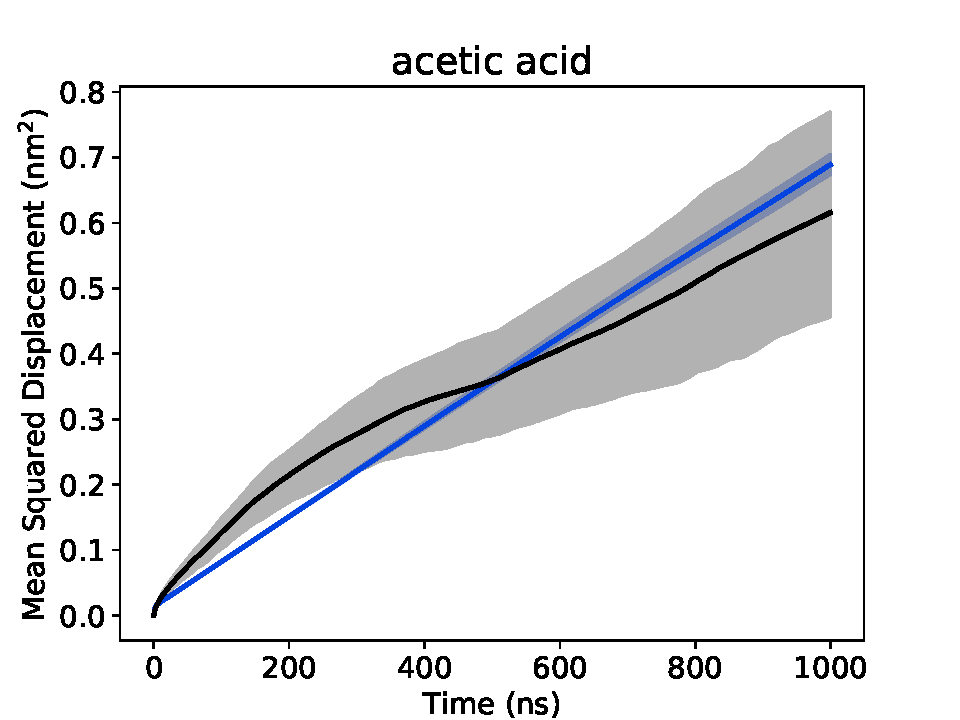
\includegraphics[width=\textwidth]{msd_ACH.pdf}
  \caption{}\label{fig:msd_ACH}
  \end{subfigure}
  \caption{The MSDs predicted based on 1000 realizations of our model (blue) tend to underpredict
  the MSDs based on the MD trajectories (black). Due to the variability in solute behavior across MD trajectories,
  as demonstrated in Figure~\ref{fig:trajectory_realizations_MET}, there are several 
  individual solute MSD curves that are significantly higher than the rest and drive up the
  mean of the MSD. If we remove those trajectories from the MSD calculation, we obtain 
  estimates much closer to the IHMM estimate.(I haven't done it yet, but could plot a third curve
  with outlier removed). Acetic acid, has no obvious outliers which is consistent with our model's
  prediction which lies within the 1$\sigma$ confidence interval of MD after a 1000 ns time lag.}\label{fig:msds}
  \end{figure}
  
  % BJC3: maybe need to talk about the curvature. Our model shouldn't have noticeable
  % curvature because it's only correlated with one step
  
  \subsection{Estimating Solute Flux and Selectivity}  
  
  %BJC3: I still need to implement this into my mean first passage time code, but it will very closely follow the 
  % methodology of the last paper. However, if I see that the decay in flux is
  % near 2 (which I expect), then I may add a short section showing how you can
  % simply use the ratio of the MSD slopes in order to estimate selectivity.
  % I think they should give the same results. Haven't tested it yet though. 
  %BJC5: currently running these simulations then will write this section up. 
  
  We can use realizations of our model in order to predict macropscopic flux and
  selectivity.
  \begin{itemize}
    \item For various length pores, we constructed distributions of first passage times for each solute and
    fit them to Equation~\ref{eqn:passage_times} in order estimate the mean 
    first passage time (MFPT). 
    \item We plotted the inverse of MFPT, the solute flux, versus pore length
    in Figure TBD.
    \item Flux rapdily decays with pore length.
    \item Selectivity is simply the ratio of the fluxes for this system.
  \end{itemize}

  %BJC3: this paragraph is speculative.
  We can use the slopes of the MSD curves to estimate selectivity in a simpler way.
  \begin{itemize}
  	\item As in our previous work, we fit the flux curves to a decaying power law function
  	of the form:
  	\begin{equation}
    	Ae^{-\beta}
  	\end{equation}
  	\item We find that in all cases, $\beta$ is equal to 2. This is consistent with Brownian
	motion which implies long term linear behavior of the MSD curves. 
	\item Since the diffusion constant is linearly proportional to the slope of the MSD, and 
	selectivity in this system can be estimated as the ratio of diffusion constants, we can 
	estimate selectivity directly based on the slopes of our stochastically simulated MSD curves.
  \end{itemize}
  
  \section{Conclusion}
  
  \noindent We have shown that the IHMM can be used to parameterize solute time series
  with an unknown number of latent dynamical modes. \\
  
  \noindent We showcase this modeling approach by example, but it is important to
  recognize the generality of this analysis.
  
  \noindent We can use the IHMM to help identify mechanisms by relating the latent
  states to observed solute behavior. \\
  
  \noindent We show how one can use the IHMM to predict macroscopic transport properties. \\
  
  \section*{Supporting Information}

  Detailed explanations and expansions upon the results and procedures mentioned in
  the main text are described in the Supporting Information. This information is
  available free of charge via the Internet at http://pubs.acs.org.

  \section*{Acknowledgements}

  %MRS2: add GAANN and PRF here to cover bases.
  This work was supported in part by the ACS Petroleum Research Fund
  grant \#59814-ND7 and the Graduate Assistance in Areas of National Need (GAANN) 
  fellowship which is funded by the U.S. Department of Education. 
  Molecular simulations were performed using the Extreme Science and
  Engineering Discovery Environment (XSEDE), which is supported by National
  Science Foundation grant number ACI-1548562. Specifically, it used the Bridges
  system, which is supported by NSF award number ACI-1445606, at the Pittsburgh
  Supercomputing Center (PSC). This work also utilized the RMACC Summit supercomputer,
  which is supported by the National Science Foundation (awards ACI-1532235 and
  ACI-1532236), the University of Colorado Boulder, and Colorado State
  University. The Summit supercomputer is a joint effort of the University of
  Colorado Boulder and Colorado State University.

  \clearpage

  \bibliographystyle{ieeetr}
  \bibliography{hdphmm}

  %\newpage

  %\section*{TOC Graphic}

\end{document}
